\section[Microeconomic Foundations: Competitive Markets, Welfare, Monopoly, Price Discrimination]{Microeconomic Foundations: Competitive Markets, Welfare,\\ Monopoly, Price Discrimination}

This appendix collects the partial-equilibrium microeconomics used throughout the notes: how a price-taking firm chooses output, how a market and an industry with free entry reach equilibrium, why competitive equilibrium maximizes total surplus, how taxes create deadweight loss, how a monopolist sets price, and how price discrimination changes output and welfare. Everything is static (one period) and, unless stated otherwise, goods are perfectly divisible.

\paragraph{Calculus facts used in this appendix.}
\begin{itemize}
\item \textbf{Chain rule:} if $y=y(p)$ then $\frac{d}{dp}f(y(p))=f'(y(p))\,y'(p)$.
\item \textbf{Implicit differentiation:} if an equation $G(p,m)=0$ defines $p$ as a function of $m$, differentiate both sides with respect to $m$ (treating $p=p(m)$) and solve for $p'(m)$.
\item \textbf{Comparative statics of an optimum:} if $y^*(c)$ solves $\max_y \pi(y,c)$, with FOC $\pi_y(y^*(c),c)=0$ and SOC $\pi_{yy}<0$, then differentiating the FOC in $c$ gives $\pi_{yy}\,\frac{dy^*}{dc}+\pi_{yc}=0$, i.e.\ $\frac{dy^*}{dc}=-\frac{\pi_{yc}}{\pi_{yy}}$.
\item \textbf{Concavity inequality:} a differentiable concave function lies below each of its tangent planes: $u(x')\le u(x^0)+\nabla u(x^0)\cdot(x'-x^0)$ for all $x',x^0$.
\item \textbf{Price elasticity of demand:} $\epsilon=\frac{dy}{dp}\frac{p}{y}$ (percentage change in quantity per 1\% change in price); $\epsilon<0$ for downward-sloping demand, and we write $|\epsilon|=-\epsilon$. Demand is \emph{elastic} if $|\epsilon|>1$, \emph{inelastic} if $|\epsilon|<1$.
\end{itemize}

%======================================================================
\subsection{The competitive firm and its supply curve \pg{45}}

\paragraph{Setup.}
\begin{itemize}
\item One good, produced in quantity $y\ge 0$ by a single firm.
\item $c(y)$: total cost of producing $y$. It splits as $c(y)=c_v(y)+F$, where $c_v(y)$ is variable cost (with $c_v(0)=0$) and $F\ge 0$ is a fixed cost that must be paid even if $y=0$ (short run).
\item Cost concepts: marginal cost $MC=c'(y)$; average cost $AC=c(y)/y$; average variable cost $AVC=c_v(y)/y$. Note $AC-AVC=F/y$.
\item $\bar p$: the market price. A \textbf{competitive firm} takes $\bar p$ as given and outside its control (it is a \emph{price-taker}).
\end{itemize}

Because consumers can buy from many other sellers at $\bar p$, the demand curve facing an ideal competitive firm is
\[
D(p)=\begin{cases}0 & \text{if } p>\bar p \quad(\text{no consumer pays more than the market price}),\\[2pt] \text{any amount} & \text{if } p=\bar p,\\[2pt] \infty & \text{if } p<\bar p \quad(\text{everyone would buy from this firm}).\end{cases}
\]
So the firm effectively sells any quantity it likes at $p=\bar p$; we write $p$ for that given price below.

\paragraph{Profit maximization.} The firm chooses $y$ to solve
\begin{equation}\label{eq:micro-cf}
\max_{y\ge 0}\ \pi(y)=p\,y-c(y).
\end{equation}
Differentiate with respect to $y$ and set to zero:
\begin{align*}
\pi'(y)&=p-c'(y)=0 &&\text{(first-order condition, FOC)}\\
\Longrightarrow\quad p&=c'(y^*). &&\text{(price = marginal cost)}
\end{align*}
The second-order condition (SOC) for a maximum is $\pi''(y^*)=-c''(y^*)\le 0$, i.e.\ $c''(y^*)\ge 0$: marginal cost must be non-decreasing at the optimum.

Read the FOC $p=c'(y)$ as a function of $y$: it gives the price at which the firm would want to supply $y$, the \textbf{inverse supply function} $p(y)=c'(y)$. Solving it for $y$ gives the supply function $y(p)$. The condition $p=MC$ is also what makes competitive output efficient (Section~\ref{sec:micro-welfare}): the price buyers pay equals the cost of the last unit.

\paragraph{1. The supply curve slopes up (interior solution).} The supply function satisfies the FOC identically in $p$:
\begin{align*}
p&=c'\big(y(p)\big) &&\text{for every } p\\
1&=c''\big(y(p)\big)\,y'(p) &&\text{(differentiate both sides w.r.t.\ $p$, chain rule)}\\
y'(p)&=\frac{1}{c''(y(p))}>0 &&\text{(divide by $c''>0$, the strict SOC).}
\end{align*}
\emph{Interpretation:} a higher price makes extra units worth producing even though each extra unit costs more (rising $MC$), so a competitive firm's supply curve has positive slope.

\paragraph{2. When is the interior solution chosen? (Shutdown condition.)} The firm can always choose $y=0$, in which case it pays only the fixed cost and earns $\pi(0)=-F$. Producing $y(p)>0$ is (weakly) better iff
\begin{align*}
p\,y(p)-c_v(y(p))-F&\ \ge\ -F &&\text{(profit from producing $\ge$ profit from shutting down)}\\
p\,y(p)-c_v(y(p))&\ \ge\ 0 &&\text{(add $F$ to both sides: $F$ is paid either way)}\\
p&\ \ge\ \frac{c_v(y(p))}{y(p)}=AVC(y(p)) &&\text{(divide by $y(p)>0$).}
\end{align*}
Combined with $p=MC$, the firm produces a positive amount only where $MC\ge AVC$.

\begin{keybox}[title=Short-run supply of a competitive firm]
\[
y(p)=\begin{cases}0 & \text{if } p<\min AVC,\\ \text{the solution of } p=c'(y) \text{ on the rising part of } MC & \text{if } p\ge \min AVC.\end{cases}
\]
The fixed cost $F$ does not affect the shutdown decision, because it is paid whether or not the firm produces.
\end{keybox}

\begin{center}
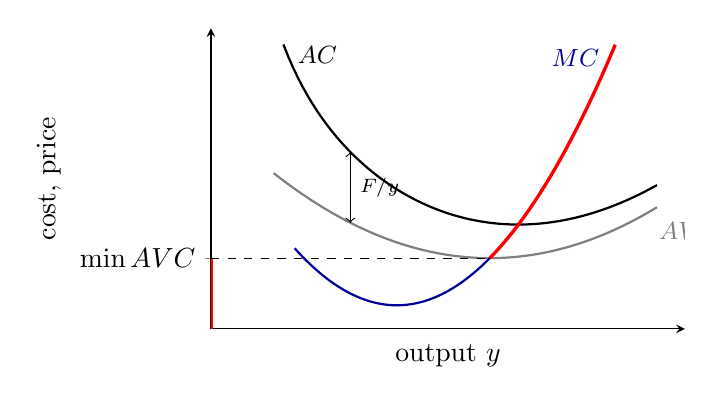
\begin{tikzpicture}
\begin{axis}[width=7.6cm,height=5.4cm,axis lines=left,xmin=0,xmax=3.4,ymin=0,ymax=8.5,
  xlabel={output $y$},ylabel={cost, price},xtick=\empty,ytick={2},yticklabels={$\min AVC$},
  domain=0.45:3.2,samples=80,restrict y to domain=0:8.3,clip=true]
\addplot[thick,black]{x^2-4*x+6+2/x} node[pos=0.04,right]{\small $AC$};
\addplot[thick,gray]{x^2-4*x+6} node[pos=0.97,below right]{\small $AVC$};
\addplot[thick,blue!60!black,domain=0.6:2.9]{3*x^2-8*x+6} node[pos=0.96,left]{\small $MC$};
\addplot[very thick,red,domain=2:2.9]{3*x^2-8*x+6};
\draw[very thick,red] (axis cs:0,0)--(axis cs:0,2);
\draw[dashed] (axis cs:0,2)--(axis cs:2,2);
\draw[<->,thin] (axis cs:1,3.0)--(axis cs:1,5.0) node[midway,right]{\scriptsize $F/y$};
\end{axis}
\end{tikzpicture}
\end{center}
\textit{How to read the figure.} Output is on the horizontal axis and cost per unit (or price) on the vertical axis. $AVC$ and $AC$ are U-shaped and $MC$ cuts both at their minima (when marginal cost is below an average, it pulls the average down; when above, it pulls it up). The vertical gap between $AC$ and $AVC$ is $F/y$, which shrinks as $y$ grows. The firm's supply curve is drawn in red: zero output (the vertical axis) for prices below $\min AVC$, and the $MC$ curve above its intersection with $AVC$.

%======================================================================
\subsection{Industry supply, market equilibrium, entry and exit \pg{46}}

\paragraph{Setup.}
\begin{itemize}
\item $n$ consumers, $i=1,\dots,n$, with individual demand functions $x_i(p)$; market demand $X(p)=\sum_{i=1}^n x_i(p)$, with $X'(p)<0$.
\item $m$ competitive firms, $j=1,\dots,m$, with supply functions $y_j(p)$ from the previous subsection, $y_j'(p)>0$.
\item \textbf{Industry supply} is the horizontal sum of firm supplies: $Y(p)=\sum_{j=1}^m y_j(p)$.
\end{itemize}

\paragraph{Market equilibrium.} The equilibrium price $p^*$ equates industry demand and industry supply:
\begin{equation}\label{eq:micro-mkteq}
\sum_{i=1}^{n} x_i(p^*)=\sum_{j=1}^{m} y_j(p^*).
\end{equation}

\paragraph{Effect of the number of firms on the price.} Let all $m$ firms be identical with supply $y(p)$, so industry supply is $m\,y(p)$ and \eqref{eq:micro-mkteq} becomes
\[
X(p)=m\,y(p).
\]
This equation defines the equilibrium price as an implicit function $p(m)$ of the number of firms. Differentiate both sides with respect to $m$ (product rule on the right, chain rule on both sides):
\begin{align*}
X'(p)\,p'(m)&=y(p)+m\,y'(p)\,p'(m) \\
X'(p)\,p'(m)-m\,y'(p)\,p'(m)&=y(p) &&\text{(collect the $p'(m)$ terms)}\\
p'(m)&=\frac{y(p)}{X'(p)-m\,y'(p)} &&\text{(divide by $X'(p)-m\,y'(p)$).}
\end{align*}
\emph{Sign:} the numerator $y(p)>0$; in the denominator $X'(p)<0$ and $-m\,y'(p)<0$, so the denominator is negative. Hence $p'(m)<0$. Each firm's output then changes by
\[
\frac{d\,y(p(m))}{dm}=y'(p)\,p'(m)<0 \qquad(\text{positive}\times\text{negative}).
\]
\emph{Interpretation:} more firms shift industry supply out, which lowers the market price, and each firm responds to the lower price by producing less ($m\uparrow\Rightarrow p\downarrow\Rightarrow y\downarrow$).

\paragraph{Entry and exit (long run).} In the long run the number of firms $m$ is variable. Assume there are no costs of entering or exiting and that potential entrants have the same cost function $c(y)$ as incumbents.
\begin{itemize}
\item If incumbents earn positive profit, new firms enter; each entrant adds its supply, so the industry supply curve becomes flatter and the price falls.
\item If firms make losses, some exit, and the price rises.
\item Entry stops when profit is zero: $p\,y-c(y)=0$, i.e.\ $p=AC(y)$. At the same time each firm sets $p=MC(y)$. Both hold only where $MC=AC$, which is the bottom of the $AC$ curve.
\end{itemize}

\begin{keybox}[title=Long-run competitive equilibrium with free entry]
\[
p^*=MC(y^*)=AC(y^*)=\min_y AC(y)\qquad(\text{break-even price}).
\]
When $m$ can be large, the long-run industry supply curve is (approximately) flat at $p^*$; demand determines only total quantity and hence the number of firms.
\end{keybox}

\paragraph{Example.} Let $c(y)=y^2+1$ (so $F=1$, $c_v(y)=y^2$). Then
\begin{align*}
AC(y)&=\frac{y^2+1}{y}=y+\frac1y, \qquad MC(y)=2y.\\
y+\frac1y&=2y &&\text{(break-even: set $AC=MC$)}\\
\frac1y&=y\ \Longrightarrow\ y^2=1\ \Longrightarrow\ y^*=1 &&\text{(subtract $y$; multiply by $y>0$)}\\
p^*&=MC(1)=2. &&\text{(and indeed $AC(1)=1+1=2$)}
\end{align*}
Each firm's supply is $y(p)=p/2$ (from $p=2y$), so with $m$ firms industry supply is $Y=m\,p/2$, i.e.\ the line $p=2Y/m$ through the origin, flatter for larger $m$. Firms keep entering as long as entry does not drive the equilibrium price below $2$. For instance, with market demand $p=8-Y$: $m=6$ firms give $8-Y=Y/3\Rightarrow Y=6$, $p=2$, each firm produces $1$ and earns zero profit; a seventh firm would push the price to $16/9<2$ and make every firm lose money.

\begin{center}
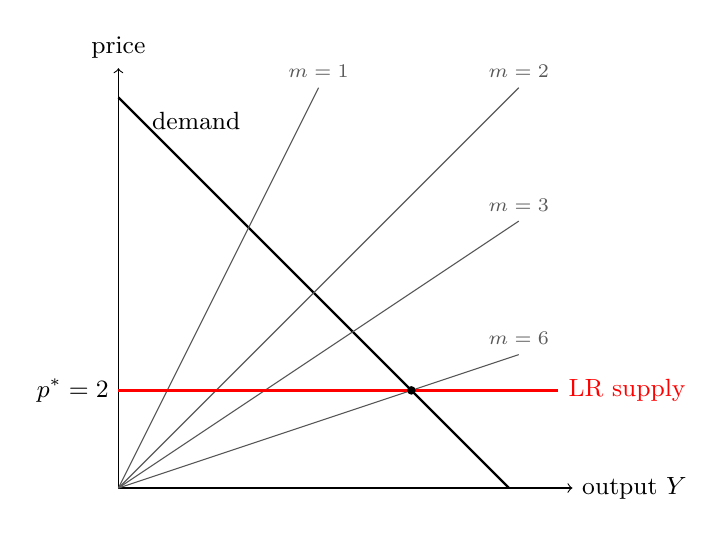
\begin{tikzpicture}[scale=0.62]
\draw[->] (0,0)--(9.3,0) node[right]{\small output $Y$};
\draw[->] (0,0)--(0,8.6) node[above]{\small price};
\draw[thick] (0,8)--(8,0) node[pos=0.06,right]{\small demand};
\foreach \m/\lab in {1/1,2/2,3/3,6/6}{
  \draw[gray!70!black] (0,0)--({min(8.2,4.1*\m)},{min(8.2,4.1*\m)*2/\m}) node[above,font=\scriptsize]{$m=\lab$};
}
\draw[very thick,red] (0,2)--(9,2) node[right]{\small LR supply};
\node[left] at (0,2) {\small $p^*=2$};
\fill (6,2) circle (2.5pt);
\end{tikzpicture}
\end{center}
\textit{How to read the figure.} Each grey ray is industry supply $p=2Y/m$ with $m$ firms; adding firms rotates it down (flatter). The demand line crosses successive rays at lower and lower prices. Entry continues until the crossing reaches the break-even price $p^*=2$ (here at $m=6$), so the long-run supply curve is the horizontal red line at $\min AC$.

%======================================================================
\subsection{Welfare: surplus and Pareto efficiency \pg{47--48}}\label{sec:micro-welfare}

\paragraph{Setup (one representative consumer).}
\begin{itemize}
\item Two goods: the $x$-good (the good being studied) and the $y$-good (``money'', all other goods), with the price of $y$ normalized to $1$.
\item \textbf{Quasilinear utility} $U(x,y)=u(x)+y$, with $u'>0$, $u''<0$, $u(0)=0$.
\item The consumer is endowed with $w$ units of the $y$-good. Producing $x$ units of the $x$-good uses up $c(x)$ units of the $y$-good ($c'>0$, $c''\ge 0$), so what is left to consume is $y=w-c(x)$.
\end{itemize}

\paragraph{The efficient quantity.} Choose $x$ to maximize utility:
\begin{align*}
&\max_{x,y}\ u(x)+y\quad\text{s.t.}\quad y=w-c(x)\\
\Longleftrightarrow\ &\max_x\ u(x)+w-c(x) &&\text{(substitute the constraint)}\\
\Longrightarrow\ & u'(x^*)=c'(x^*). &&\text{(FOC; $w$ is a constant)}
\end{align*}
The SOC $u''-c''<0$ holds by the assumptions.

\paragraph{Surplus interpretation.} With quasilinear utility, utility maximization at price $p$ gives $u'(x)=p$, so the inverse demand curve is the marginal-utility curve $u'(x)$; the competitive (inverse) supply curve is the marginal-cost curve $c'(x)$. Then, using $u(0)=0$:
\[
u(x)=\int_0^x u'(s)\,ds=\text{area under demand},\qquad c(x)-c(0)=\int_0^x c'(s)\,ds=\text{area under supply}.
\]
(Fixed costs $c(0)$ do not depend on $x$ and are ignored in what follows.) Define
\begin{align*}
CS(x)&=u(x)-p\,x &&\text{(consumer surplus: value minus amount paid)}\\
PS(x)&=p\,x-c(x) &&\text{(producer surplus = profit)}\\
CS(x)+PS(x)&=u(x)-p\,x+p\,x-c(x)=u(x)-c(x) &&\text{(payments $px$ cancel: a transfer).}
\end{align*}
So maximizing $u(x)-c(x)$ is the same as maximizing total surplus, the area under the demand curve and above the supply curve.

\begin{keybox}[title=First welfare result (partial equilibrium)]
In competitive equilibrium consumers set $u'(x)=p^*$ and firms set $c'(x)=p^*$, so $u'(x^*)=c'(x^*)$: the competitive output is exactly the one that maximizes total surplus $u(x)-c(x)$.
\end{keybox}

\begin{center}
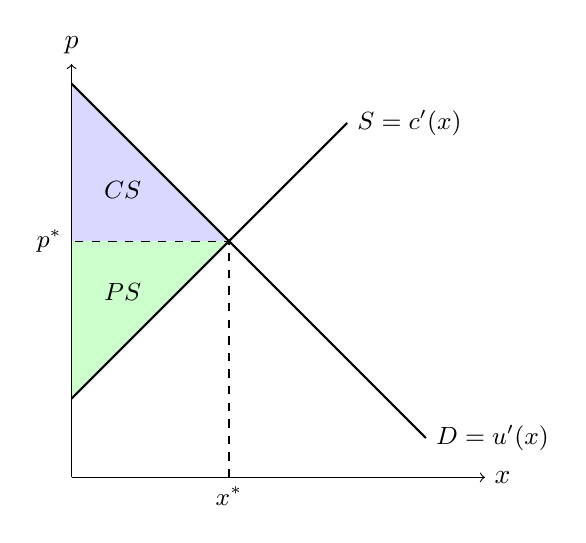
\begin{tikzpicture}[scale=0.5]
\fill[blue!15] (0,10)--(0,6)--(4,6)--cycle;
\fill[green!20] (0,6)--(0,2)--(4,6)--cycle;
\draw[->] (0,0)--(10.5,0) node[right]{$x$};
\draw[->] (0,0)--(0,10.5) node[above]{$p$};
\draw[thick] (0,10)--(9,1) node[right]{\small $D=u'(x)$};
\draw[thick] (0,2)--(7,9) node[right]{\small $S=c'(x)$};
\draw[dashed] (4,0) node[below]{\small $x^*$}--(4,6)--(0,6) node[left]{\small $p^*$};
\node at (1.3,7.3) {\small $CS$};
\node at (1.3,4.7) {\small $PS$};
\end{tikzpicture}
\end{center}
\textit{How to read the figure.} Demand slopes down because marginal utility diminishes; supply slopes up because marginal cost rises. Consumer surplus (blue) is the area between demand and the price line; producer surplus (green) is the area between the price line and supply. Their sum, the triangle between demand and supply up to $x^*$, is total surplus. Stopping at any $x<x^*$ would forgo units whose value $u'$ exceeds their cost $c'$; going beyond $x^*$ would produce units that cost more than they are worth.

\paragraph{Several consumers and firms.}
\begin{itemize}
\item Consumers $i=1,\dots,n$: utility $u_i(x_i)+y_i$, endowment $w_i$ of the $y$-good.
\item Firms $j=1,\dots,m$: firm $j$ produces $z_j$ units of the $x$-good at cost $c_j(z_j)$ (in units of the $y$-good).
\item Feasibility: total $x$ consumed equals total produced, $\sum_i x_i=\sum_j z_j$; total $y$ consumed equals endowments minus resources used in production, $\sum_{i=1}^n y_i=\sum_{i=1}^n w_i-\sum_{j=1}^m c_j(z_j)$.
\end{itemize}
A planner maximizes the sum of utilities $\sum_{i=1}^n u_i(x_i)+\sum_{i=1}^n y_i$. Substituting the $y$-feasibility condition:
\begin{equation}\label{eq:micro-planner}
\max_{\{x_i\},\{z_j\}}\ \sum_{i=1}^n u_i(x_i)+\sum_{i=1}^n w_i-\sum_{j=1}^m c_j(z_j)\quad\text{s.t.}\quad \sum_{i=1}^n x_i=\sum_{j=1}^m z_j .
\end{equation}
Lagrangian with multiplier $\lambda$ on the constraint:
\[
\mathcal L=\sum_i u_i(x_i)+\sum_i w_i-\sum_j c_j(z_j)+\lambda\Big(\sum_j z_j-\sum_i x_i\Big).
\]
FOCs:
\begin{align*}
\frac{\partial\mathcal L}{\partial x_i}&=u_i'(x_i^*)-\lambda=0\ \Longrightarrow\ u_i'(x_i^*)=\lambda\quad\text{for all } i,\\
\frac{\partial\mathcal L}{\partial z_j}&=-c_j'(z_j^*)+\lambda=0\ \Longrightarrow\ c_j'(z_j^*)=\lambda\quad\text{for all } j.
\end{align*}
These are exactly the competitive equilibrium conditions with $p^*=\lambda$: each consumer sets $u_i'(x_i)=p^*$, each firm sets $c_j'(z_j)=p^*$. \emph{Interpretation:} the equilibrium price acts as the shadow value of the $x$-good, equating every consumer's marginal utility with every firm's marginal cost, which is what the planner wants.

\paragraph{Pareto efficiency.} A more general welfare criterion than ``sum of utilities'' is Pareto efficiency.
\begin{itemize}
\item An allocation is \textbf{Pareto efficient} if there is no other feasible allocation that makes some agent better off without making any agent worse off.
\end{itemize}
To characterize it, take two agents and total resources $\bar x$, $\bar y$ (so $x_2=\bar x-x_1$, $y_2=\bar y-y_1$). An allocation is Pareto efficient iff it maximizes agent 1's utility holding agent 2's utility at some level $\bar u$:
\begin{align*}
&\max_{x_1,y_1}\ u_1(x_1)+y_1\quad\text{s.t.}\quad u_2(\bar x-x_1)+\bar y-y_1=\bar u\\
&y_1=u_2(\bar x-x_1)+\bar y-\bar u &&\text{(solve the constraint for $y_1$)}\\
&\max_{x_1}\ u_1(x_1)+u_2(\bar x-x_1)+(\bar y-\bar u) &&\text{(substitute; $\bar y-\bar u$ is a constant)}\\
&u_1'(x_1)-u_2'(\bar x-x_1)=0 &&\text{(FOC, chain rule on $u_2$)}.
\end{align*}
\begin{keybox}[title=Necessary condition for Pareto efficiency (quasilinear case)]
\[
u_1'(x_1)=u_2'(x_2),\qquad x_2=\bar x-x_1:
\]
marginal utilities of the $x$-good (in units of money) are equalized across agents. So, essentially, Pareto efficiency requires maximizing $u_1(x_1)+u_2(x_2)$.
\end{keybox}
\emph{Interpretation:} if agent 1's marginal utility were higher, moving a little $x$ from agent 2 to agent 1, and having agent 1 hand agent 2 just enough $y$ to compensate, would leave agent 2 indifferent and agent 1 strictly better off. In competitive equilibrium every consumer sets $u_i'(x_i)=p^*$, so the marginal utilities are automatically equal and the equilibrium is Pareto efficient.

\begin{tipbox}
With quasilinear utility, the way the $y$-good (``money'') is divided does not affect efficiency: the efficiency condition pins down only the allocation of $x$. Moving $y$ between people is pure redistribution: it changes fairness (equity), not efficiency.
\end{tipbox}

%======================================================================
\subsection{Taxes and subsidies \pg{49}}

\paragraph{Setup.} A tax drives a wedge between two prices:
\begin{itemize}
\item $p_d$: the \textbf{demand price}, paid by buyers (including the tax);
\item $p_s$: the \textbf{supply price}, received by sellers.
\end{itemize}
The demand function is $D(\cdot)$ and supply function $S(\cdot)$; $P_d(x)$ and $P_s(x)$ are the inverse demand and inverse supply curves. Three instruments:
\begin{itemize}
\item \textbf{Quantity (unit) tax} $t$ per unit sold: $p_d=p_s+t$.
\item \textbf{Value (ad valorem) tax} at rate $\tau$ on expenditure: $p_d=(1+\tau)\,p_s$.
\item \textbf{Quantity subsidy} $s$ per unit: the seller receives $s$ more per unit than the buyer pays, so $p_d=p_s-s$.
\end{itemize}

\paragraph{Equilibrium.} Buyers respond to $p_d$, sellers to $p_s$, and quantity demanded must equal quantity supplied:
\[
D(p_d)=S(p_s),\qquad p_d=p_s+t .
\]
Equivalently, with inverse curves, the equilibrium quantity $x_t$ solves
\[
P_d(x_t)=P_s(x_t)+t\qquad\big(\text{or } P_s(x_t)=P_d(x_t)-t\big),
\]
and then $p_d=P_d(x_t)$, $p_s=P_s(x_t)$. Since $P_d$ falls and $P_s$ rises in $x$, a positive $t$ requires a smaller $x$: $x_t<x^*$, where $x^*$ is the no-tax quantity ($P_d(x^*)=P_s(x^*)$).

\paragraph{Welfare with the tax.} At the post-tax quantity $x_t$ (with $u$ and $c$ as in Section~\ref{sec:micro-welfare}):
\begin{align*}
CS&=u(x_t)-p_d\,x_t &&\text{(buyers pay $p_d$)}\\
PS&=p_s\,x_t-c(x_t) &&\text{(sellers receive $p_s$)}\\
T&=t\,x_t=(p_d-p_s)\,x_t &&\text{(tax revenue, returned to society)}\\
W(x_t)=CS+PS+T&=u(x_t)-p_dx_t+p_sx_t-c(x_t)+(p_d-p_s)x_t\\
&=u(x_t)-c(x_t). &&\text{(all payments cancel)}
\end{align*}
Tax revenue must be counted as part of welfare: it is a transfer from buyers and sellers to the government, not a loss.

\begin{keybox}[title=Deadweight loss]
\[
DWL=W(x^*)-W(x_t)=\int_{x_t}^{x^*}\big[u'(s)-c'(s)\big]\,ds>0 .
\]
It is the surplus from the trades between $x_t$ and $x^*$ that no longer happen, although buyers valued those units above their cost of production.
\end{keybox}

\begin{center}
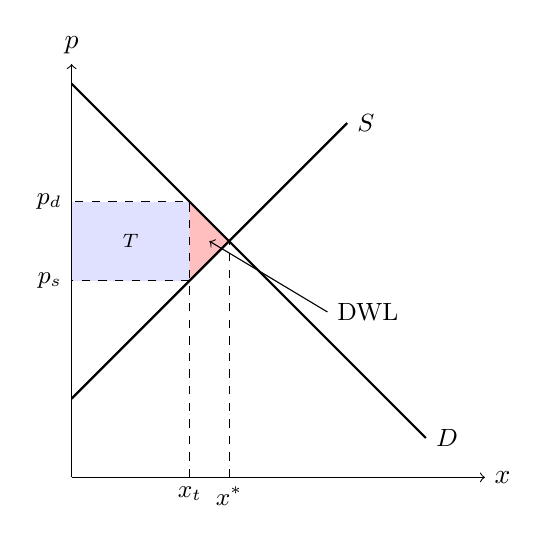
\begin{tikzpicture}[scale=0.5]
\fill[blue!12] (0,5) rectangle (3,7);
\fill[red!25] (3,7)--(3,5)--(4,6)--cycle;
\draw[->] (0,0)--(10.5,0) node[right]{$x$};
\draw[->] (0,0)--(0,10.5) node[above]{$p$};
\draw[thick] (0,10)--(9,1) node[right]{\small $D$};
\draw[thick] (0,2)--(7,9) node[right]{\small $S$};
\draw[dashed] (3,0) node[below]{\small $x_t$}--(3,7)--(0,7) node[left]{\small $p_d$};
\draw[dashed] (3,5)--(0,5) node[left]{\small $p_s$};
\draw[dashed] (4,0) node[below]{\small $x^*$}--(4,6);
\node at (1.5,6) {\scriptsize $T$};
\draw[<-] (3.5,6)--(6.5,4.2) node[right]{\small DWL};
\end{tikzpicture}
\end{center}
\textit{How to read the figure.} Without the tax the market clears at $x^*$. With a unit tax $t$, the quantity $x_t$ is where the vertical gap between demand and supply equals $t$: buyers pay $p_d$, sellers get $p_s=p_d-t$. The blue rectangle (height $t$, width $x_t$) is tax revenue $T$, a transfer. The red triangle between $x_t$ and $x^*$ is the deadweight loss: surplus that nobody receives.

%======================================================================
\subsection{Monopoly: the pricing rule \pg{50--52}}

\paragraph{Setup.}
\begin{itemize}
\item A single seller (the \textbf{monopolist}) with cost function $c(y)$, $c'>0$.
\item Market demand $D(p)$, downward sloping; its inverse $p(y)$ (the price at which consumers buy exactly $y$) satisfies $p'(y)<0$.
\item Revenue $r(y)=p(y)\,y$; marginal revenue $MR=r'(y)$.
\end{itemize}
A monopolist has market power: the amount it can sell responds \emph{continuously} to the price it charges. Contrast the competitive firm, whose sales drop to zero if it charges above the market price. A competitive firm is a price-taker; a monopolist is a \textbf{price-maker}.

\paragraph{The problem.} The monopolist faces two constraints, technology ($c(y)$) and consumer behaviour (it cannot sell more than is demanded):
\[
\max_{p,\,y}\ p\,y-c(y)\quad\text{s.t.}\quad D(p)\ge y .
\]
It would never produce output it cannot sell, so the constraint binds, $y=D(p)$. The problem can be written in terms of price, $\max_p\ p\,D(p)-c(D(p))$, or, more conveniently, using the inverse demand curve, in terms of quantity:
\begin{equation}\label{eq:micro-monop}
\max_y\ \pi(y)=p(y)\,y-c(y).
\end{equation}
Differentiate (product rule on $p(y)\,y$):
\begin{align}
\text{FOC:}\quad & \underbrace{p(y)+p'(y)\,y}_{MR=r'(y)}=\underbrace{c'(y)}_{MC}, \label{eq:micro-mrmc}\\
\text{SOC:}\quad & \pi''(y)=2p'(y)+p''(y)\,y-c''(y)\le 0. \notag
\end{align}

\paragraph{Why marginal revenue is below price.} When the monopolist considers selling $dy$ more units there are two effects:
\begin{itemize}
\item revenue rises by $p\,dy$ from selling the extra units at the current price;
\item but to sell them it must cut the price by $dp=p'(y)\,dy<0$ on all $y$ units it already sells.
\end{itemize}
So $dr=p\,dy+y\,dp=\big[p+p'(y)\,y\big]\,dy$. Since $p'(y)<0$, $MR<p(y)$ for every $y>0$, while at $y=0$, $MR=p(0)$: the first unit costs no price cut on earlier units. Hence the $MR$ curve starts at the demand intercept and lies below the inverse demand curve.

The SOC says that the slope of $MR$, $2p'+p''y$, is less than the slope of $MC$, $c''$: the $MR$ curve cuts the $MC$ curve \emph{from above}.

\paragraph{Elasticity form of the FOC.} Factor $p(y)$ out of $MR$:
\begin{align*}
r'(y)&=p(y)\Big[1+\frac{dp}{dy}\,\frac{y}{p}\Big] &&\text{(factor out $p$)}\\
&=p(y)\Big[1+\frac{1}{\epsilon(y)}\Big], &&\epsilon(y)=\frac{p}{y}\frac{dy}{dp}\ \text{(so }\tfrac{dp}{dy}\tfrac{y}{p}=\tfrac{1}{\epsilon}\text{)}\\
&=p(y)\Big[1-\frac{1}{|\epsilon(y)|}\Big] &&\text{(since $\epsilon<0$, $\epsilon=-|\epsilon|$).}
\end{align*}
So the FOC \eqref{eq:micro-mrmc} reads
\begin{equation}\label{eq:micro-markup}
p(y)\Big[1-\frac{1}{|\epsilon(y)|}\Big]=c'(y).
\end{equation}
\emph{Demand must be elastic at the optimum.} If $|\epsilon(y)|<1$, the bracket is negative, so $MR<0<MC$: cutting output would raise revenue \emph{and} lower cost. Hence at the monopoly optimum $|\epsilon(y)|\ge 1$ (strictly $>1$ when $MC>0$), i.e.\ $\epsilon(y)<-1$.

\begin{keybox}[title=Monopoly markup rule]
Solving \eqref{eq:micro-markup} for $p$:
\[
p=\frac{c'(y)}{1-1/|\epsilon|}.
\]
Price is a markup over marginal cost; the markup is larger the less elastic is demand, and goes to zero (price $\to MC$) as $|\epsilon|\to\infty$, the competitive case.
\end{keybox}

\paragraph{Special case 1: linear demand.} Let $p(y)=a-by$ ($a,b>0$) and constant marginal cost, $c(y)=cy$ with $c<a$.
\begin{align*}
r(y)&=ay-by^2,\qquad r'(y)=a-2by &&\text{($MR$ is twice as steep as demand)}\\
a-2by^*&=c &&\text{(set $MR=MC$)}\\
y^*&=\frac{a-c}{2b} &&\text{(solve for $y$)}\\
p^*&=a-b\,\frac{a-c}{2b}=\frac{a+c}{2}. &&\text{(substitute into demand)}
\end{align*}
For comparison, the competitive outcome $p=c$ gives $y_c=(a-c)/b=2y^*$: the monopolist produces half the competitive output.

\paragraph{Special case 2: constant-elasticity demand.} Let $y=A\,p^{-b}$ with $A>0$, $b>1$. Then
\[
\epsilon=\frac{p}{y}\frac{dy}{dp}=\frac{p}{Ap^{-b}}\cdot(-b)A\,p^{-b-1}=-b,
\]
constant at every point. With constant marginal cost $c$, \eqref{eq:micro-markup} gives
\[
p=\frac{c}{1-1/b}=\frac{b}{b-1}\,c,
\]
a \emph{constant} markup over marginal cost whose size depends only on the elasticity of demand.

\begin{center}
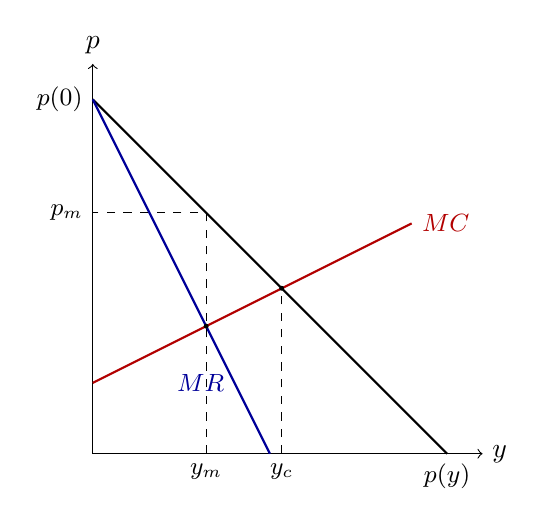
\begin{tikzpicture}[scale=0.45]
\draw[->] (0,0)--(11,0) node[right]{$y$};
\draw[->] (0,0)--(0,11) node[above]{$p$};
\draw[thick] (0,10) node[left]{\small $p(0)$}--(10,0) node[below]{\small $p(y)$};
\draw[thick,blue!60!black] (0,10)--(5,0) node[pos=0.8,left]{\small $MR$};
\draw[thick,red!70!black] (0,2)--(9,6.5) node[right]{\small $MC$};
\draw[dashed] (3.2,0) node[below]{\small $y_m$}--(3.2,6.8)--(0,6.8) node[left]{\small $p_m$};
\draw[dashed] (5.33,0) node[below]{\small $y_c$}--(5.33,4.67);
\fill (3.2,3.6) circle (2pt);
\fill (5.33,4.67) circle (2pt);
\end{tikzpicture}
\end{center}
\textit{How to read the figure.} Inverse demand $p(y)$ is the consumers' marginal willingness to pay; $MR$ starts at the same intercept $p(0)$ and falls twice as fast (linear case). The monopolist produces $y_m$ where $MR$ crosses $MC$ from above, then charges the highest price consumers will pay for $y_m$, read off the demand curve: $p_m$. The competitive output $y_c$ is where demand meets $MC$; since $MR$ lies below demand, $y_m<y_c$ and $p_m>MC(y_m)$.

%======================================================================
\subsection{Monopoly: cost pass-through \pg{52--53}}

\paragraph{Question.} How do the monopolist's output and price respond when its marginal cost rises? Assume constant marginal cost $c$, so the problem is $\max_y\ \pi(y,c)=p(y)\,y-c\,y$ with FOC
\begin{equation}\label{eq:micro-foc-c}
p(y)+y\,p'(y)-c=0 .
\end{equation}

\paragraph{Output.} Let $y(c)$ solve \eqref{eq:micro-foc-c}. Differentiate the identity with respect to $c$ (chain rule; product rule on $y\,p'(y)$):
\begin{align*}
p'(y)\frac{dy}{dc}+\Big[p'(y)\frac{dy}{dc}+y\,p''(y)\frac{dy}{dc}\Big]-1&=0\\
\big[2p'(y)+y\,p''(y)\big]\frac{dy}{dc}&=1 &&\text{(collect terms)}\\
\frac{dy}{dc}&=\frac{1}{2p'(y)+y\,p''(y)}<0 .
\end{align*}
This is the general formula $\frac{dy}{dc}=-\pi_{yc}/\pi_{yy}$ with $\pi_{yc}=-1$ and $\pi_{yy}=2p'+yp''$. The denominator is the SOC (with $c''=0$), which is negative at a maximum, so $dy/dc<0$: the monopolist always cuts output when marginal cost rises.

\paragraph{Price.} Price moves along the demand curve, $p=p(y(c))$:
\begin{align*}
\frac{dp}{dc}&=p'(y)\,\frac{dy}{dc} &&\text{(chain rule)}\\
&=\frac{p'(y)}{2p'(y)+y\,p''(y)} &&\text{(substitute $dy/dc$)}\\
&=\frac{1}{2+y\,p''(y)/p'(y)} &&\text{(divide top and bottom by $p'(y)$).}
\end{align*}
It is a ratio of two negative numbers, so $dp/dc>0$. The magnitude depends on the curvature of demand, $p''$.

\paragraph{Linear demand.} $p''(y)=0$, so
\[
\frac{dp}{dc}=\frac12 .
\]
(Check with the closed form $p^*=(a+c)/2$.) The monopolist passes half of a cost increase on to consumers.

\paragraph{Constant-elasticity demand.} With $\epsilon<-1$ (write $|\epsilon|=b>1$), the markup rule gives $p=\dfrac{c}{1-1/|\epsilon|}=\dfrac{\epsilon}{1+\epsilon}\,c$, so
\[
\frac{dp}{dc}=\frac{\epsilon}{1+\epsilon}=\frac{|\epsilon|}{|\epsilon|-1}>1 .
\]
Check with the general formula: inverting $y=Ap^{-b}$ gives $p(y)=(y/A)^{-1/b}$, so
\begin{align*}
p'(y)&=-\frac1b\,\frac{p}{y},\qquad p''(y)=\frac1b\Big(\frac1b+1\Big)\frac{p}{y^2}\\
y\,\frac{p''(y)}{p'(y)}&=-\Big(\frac1b+1\Big)=-\frac{1+b}{b}\\
\frac{dp}{dc}&=\frac{1}{2-\frac{1+b}{b}}=\frac{1}{\frac{b-1}{b}}=\frac{b}{b-1}. \checkmark
\end{align*}

\begin{keybox}[title=Pass-through of a cost increase under monopoly]
\begin{itemize}
\item Linear demand: $dp/dc=1/2$ (less than full pass-through).
\item Constant elasticity: $dp/dc=|\epsilon|/(|\epsilon|-1)>1$ (more than full pass-through), because price is a constant percentage markup over cost.
\item In the constant-elasticity case, as demand becomes very elastic ($|\epsilon|\to\infty$) the markup vanishes and $dp/dc\to 1$; as demand becomes less elastic ($|\epsilon|\to 1^+$) the markup explodes and $dp/dc\to\infty$.
\end{itemize}
\end{keybox}

\begin{tipbox}
Do not confuse this with competitive tax incidence, where the side of the market with the more inelastic curve bears more of the tax. A monopolist never operates on the inelastic part of demand ($|\epsilon|<1$), and its pass-through is governed by the curvature of demand, not by elasticity alone.
\end{tipbox}

%======================================================================
\subsection{Monopoly: welfare, output and quality \pg{53--55}}

\paragraph{Quasilinear facts used here.} With $U(x,y)=u(x)+y$:
\begin{itemize}
\item $\partial U/\partial y=1$: the marginal utility of money is constant whatever the level of $y$. Hence demand for $x$ does not depend on income (a richer consumer does not buy more $x$).
\item Maximizing $u(x)+y$ s.t.\ $px+y=m$: substitute $y=m-px$, FOC $u'(x)-p=0$. So the inverse demand curve is $p(x)=u'(x)$, and $p'(x)=u''(x)<0$ when $u$ is concave.
\end{itemize}

\paragraph{Setup.} One consumer with utility $u(x)+y$; $c(x)$ is the amount of the $y$-good needed to produce $x$ units of the $x$-good. Social welfare is $W(x)=u(x)-c(x)$ (Section~\ref{sec:micro-welfare}).

\paragraph{Social optimum.} $W'(x_0)=u'(x_0)-c'(x_0)=0$, i.e.\ $u'(x_0)=p(x_0)=c'(x_0)$: price equals marginal cost at the efficient output $x_0$.

\paragraph{Monopoly output is too low.} The monopoly output $x_m$ satisfies \eqref{eq:micro-mrmc}: $p(x_m)+p'(x_m)\,x_m=c'(x_m)$. Evaluate the slope of welfare at $x_m$:
\begin{align*}
W'(x_m)&=u'(x_m)-c'(x_m)\\
&=p(x_m)-c'(x_m) &&\text{(consumer optimum: $u'=p$)}\\
&=p(x_m)-\big[p(x_m)+p'(x_m)\,x_m\big] &&\text{(monopoly FOC for $c'(x_m)$)}\\
&=-p'(x_m)\,x_m=-u''(x_m)\,x_m>0 &&\text{($u$ concave, $x_m>0$).}
\end{align*}
\emph{Interpretation:} at the monopoly output, social welfare is still increasing in $x$, so raising output from $x_m$ would raise welfare. The monopolist stops early because it counts the price cut on inframarginal units as a cost, while society counts it as a transfer to consumers.

\paragraph{Same result via $W=CS+\pi$.} Write
\[
W(x)=\underbrace{\big[u(x)-p(x)\,x\big]}_{CS(x)}+\underbrace{\big[p(x)\,x-c(x)\big]}_{\pi(x)} .
\]
At $x_m$ the monopolist maximizes profit, so $\pi'(x_m)=0$ and $W'(x_m)=CS'(x_m)$. Differentiating $CS$:
\begin{align*}
CS'(x_m)&=u'(x_m)-p(x_m)-p'(x_m)\,x_m\\
&=-p'(x_m)\,x_m>0 &&\text{(since $u'(x_m)=p(x_m)$).}
\end{align*}
Consumers, too, would like output to be increased: more output means a lower price on all units they buy.

\paragraph{Quality choice: setup.} A monopolist also chooses other product dimensions, e.g.\ \textbf{quality} $q$.
\begin{itemize}
\item Gross consumer benefit $u(x,q)$ and inverse demand $p(x,q)=u_x(x,q)$ (subscripts denote partial derivatives).
\item Cost $c(x,q)$.
\item Quality is a good and costly: $u_q>0$, $c_q>0$.
\item Social welfare $W(x,q)=u(x,q)-c(x,q)$.
\end{itemize}

\paragraph{Monopolist's choice.} $\max_{x,q}\ p(x,q)\,x-c(x,q)$, with FOCs at the optimum $(x_m,q_m)$:
\begin{align}
p(x_m,q_m)+p_x(x_m,q_m)\,x_m&=c_x(x_m,q_m), \label{eq:micro-q1}\\
x_m\,p_q(x_m,q_m)&=c_q(x_m,q_m). \label{eq:micro-q2}
\end{align}
Condition \eqref{eq:micro-q2}: the monopolist raises quality until the extra revenue (higher price on all $x_m$ units) equals the extra cost. Since $c_q>0$, it implies $p_q>0$.

\paragraph{Welfare derivatives at $(x_m,q_m)$.} By definition of $W$:
\begin{align}
\frac{\partial W}{\partial x}&=u_x(x_m,q_m)-c_x(x_m,q_m), \label{eq:micro-q3}\\
\frac{\partial W}{\partial q}&=u_q(x_m,q_m)-c_q(x_m,q_m). \label{eq:micro-q4}
\end{align}
Substitute $u_x=p$ and \eqref{eq:micro-q1} into \eqref{eq:micro-q3}:
\[
\frac{\partial W}{\partial x}=p-\big(p+p_x\,x_m\big)=-p_x(x_m,q_m)\,x_m>0 .
\]
Holding quality fixed, the monopolist produces too little output, as before. Substitute \eqref{eq:micro-q2} into \eqref{eq:micro-q4}:
\begin{equation}\label{eq:micro-q5}
\frac{\partial W}{\partial q}=\underbrace{u_q(x_m,q_m)}_{>0}-\underbrace{p_q(x_m,q_m)}_{>0\text{ by \eqref{eq:micro-q2}}}\,x_m ,
\end{equation}
a difference of two positive terms: its sign is not determined without more structure.

\paragraph{Signing \eqref{eq:micro-q5} via consumer surplus.} Write welfare as consumer surplus plus profit:
\[
W(x,q)=\underbrace{\big[u(x,q)-p(x,q)\,x\big]}_{CS(x,q)}+\underbrace{\big[p(x,q)\,x-c(x,q)\big]}_{\pi(x,q)} .
\]
Because the monopolist maximizes profit, $\partial\pi/\partial x=\partial\pi/\partial q=0$ at $(x_m,q_m)$, so there the derivatives of welfare with respect to $x$ and $q$ equal the derivatives of $CS$. Using $u(x,q)=\int_0^x p(s,q)\,ds$ (with $u(0,q)=0$):
\begin{align*}
\frac{\partial CS}{\partial q}&=u_q(x,q)-p_q(x,q)\,x\\
&=\int_0^x p_q(s,q)\,ds-\int_0^x p_q(x,q)\,ds &&\text{(differentiate under the integral; write $p_qx$ as an integral)}\\
&=\int_0^x\big[p_q(s,q)-p_q(x,q)\big]\,ds .
\end{align*}
The sign is ambiguous and depends on the cross-partial $\partial^2p/\partial x\,\partial q$:
\begin{itemize}
\item if $p_{xq}<0$ (quality raises the willingness to pay of inframarginal buyers, $s<x$, more than of the marginal buyer), the integrand is positive, $\partial W/\partial q>0$, and the monopolist under-provides quality;
\item if $p_{xq}>0$, the integrand is negative and the monopolist over-provides quality.
\end{itemize}

\paragraph{Average vs.\ marginal willingness to pay.} Another reading of \eqref{eq:micro-q5} uses the reservation-price model: think of consumers as lined up in order of decreasing willingness to pay, so $p(x,q)$ is the reservation price of consumer number $x$ (the \emph{marginal} consumer), $u(x,q)=\int_0^x p(s,q)\,ds$ is the sum of reservation prices (total willingness to pay), and $u(x,q)/x$ is the \emph{average} willingness to pay. Divide \eqref{eq:micro-q5} by $x_m$ (a constant with respect to $q$):
\[
\frac{1}{x_m}\frac{\partial W(x_m,q_m)}{\partial q}=\frac{u_q(x_m,q_m)}{x_m}-p_q(x_m,q_m)=\frac{\partial}{\partial q}\Big[\frac{u(x_m,q_m)}{x_m}-p(x_m,q_m)\Big].
\]
\begin{keybox}[title=Spence quality distortion]
The welfare gain from more quality is proportional to (change in \emph{average} willingness to pay) minus (change in \emph{marginal} willingness to pay). Society cares about all consumers' willingness to pay; the monopolist cares only about the marginal consumer's, since that sets the price. If average WTP rises faster with $q$ than marginal WTP, the monopolist supplies too little quality; in the reverse case, too much.
\end{keybox}

%======================================================================
\subsection{Price discrimination: types, setup, first and second degree \pg{56--58}}

To price-discriminate, a firm must be able to \emph{sort} consumers (know or infer who is who) and to \emph{prevent resale} (otherwise low-price buyers would resell to high-price buyers).

\begin{itemize}
\item \textbf{First degree} (perfect price discrimination): the seller charges a different price for each unit, equal to the buyer's maximum willingness to pay for that unit.
\item \textbf{Second degree} (nonlinear pricing): the price depends on the number of units bought, but not on who buys. Every consumer faces the same price schedule, but the schedule charges different amounts for different quantities (e.g.\ 3 for one unit, 5 for two; quantity discounts).
\item \textbf{Third degree}: different groups of purchasers are charged different prices (e.g.\ student or senior discounts), but within a group each buyer pays one constant price per unit.
\end{itemize}

\paragraph{Setup.}
\begin{itemize}
\item Consumers $i=1,2$ with quasilinear utility $u_i(x)+y$, normalized so that $u_i(0)=0$; $m$ denotes money income.
\item A single seller with constant marginal cost, $c(x)=cx$.
\item \textbf{Total (maximum) willingness to pay} $r_i(x)$: the largest payment for $x$ units that leaves consumer $i$ no worse off than buying nothing:
\[
u_i(0)+y=u_i(x)+y-r_i(x)\ \Longrightarrow\ r_i(x)=u_i(x)\qquad(\text{using } u_i(0)=0).
\]
So the maximum total payment for $x$ units is just the utility from $x$ units.
\item \textbf{Marginal willingness to pay} = inverse demand: maximizing $u_i(x)+y$ s.t.\ $px+y=m$ gives $u_i'(x)=p$. The price needed to induce consumer $i$ to buy $x$ is $p_i(x)=u_i'(x)$: the maximum price for the next unit.
\item Consumer 2 is the \textbf{high-demand} type, consumer 1 the low-demand type:
\[
r_2(x)>r_1(x)\ \text{ i.e. } u_2(x)>u_1(x),\quad\text{and}\quad u_2'(x)>u_1'(x)\qquad\text{for all } x>0 .
\]
\end{itemize}

\paragraph{First-degree price discrimination.} Take one consumer with utility $u(x)+y$. The monopolist makes a \textbf{take-it-or-leave-it offer} $(r,x)$: pay $r$ in total and consume $x$, or consume nothing. The consumer accepts only if he gets non-negative surplus, $u(x)-r\ge 0$. The monopolist solves
\begin{align*}
&\max_{r,\,x}\ r-cx\quad\text{s.t.}\quad u(x)\ge r .
\end{align*}
\begin{align*}
&r=u(x) &&\text{(the monopolist wants $r$ as large as possible, so the constraint binds)}\\
&\max_x\ u(x)-cx &&\text{(substitute the constraint)}\\
&u'(x^*)=c &&\text{(FOC; SOC $u''<0$ holds)}\\
&r^*=u(x^*) &&\text{(the take-it-or-leave-it price for that quantity).}
\end{align*}

\begin{keybox}[title=First-degree price discrimination]
The monopolist produces the Pareto-efficient output: marginal willingness to pay equals marginal cost, $u'(x^*)=c$, the same quantity as under perfect competition. But consumer surplus is $CS=u(x^*)-r^*=0$: the consumer is just indifferent to not buying, and the monopolist captures the entire surplus.
\begin{center}\small
\begin{tabular}{lccc}
 & total payment & $CS$ & $PS$ (profit)\\\hline
Perfect competition ($p^*=c$ per unit) & $cx^*$ & $u(x^*)-cx^*$ & $0$\\
First-degree PD & $r^*=u(x^*)$ & $0$ & $u(x^*)-cx^*$
\end{tabular}
\end{center}
\end{keybox}
\emph{Interpretation:} efficiency and distribution separate. Total surplus $u(x^*)-cx^*$ is the same in both regimes; only who gets it differs.

\paragraph{Two ways to implement it.} (i) A bundle price: sell $x^*$ for the lump sum $r^*=u(x^*)$. (ii) Sell each unit at a different price, equal to the marginal willingness to pay for that unit. To see that (ii) collects the same revenue, split $x$ into $n$ pieces of size $\Delta x$, $x=n\Delta x$. The willingness to pay $p_k$ for the $k$-th piece makes the consumer indifferent between buying it or not:
\begin{align*}
u(0)+m&=u(\Delta x)+m-p_1\ \Longrightarrow\ u(0)=u(\Delta x)-p_1 &&\text{(first piece)}\\
u(\Delta x)&=u(2\Delta x)-p_2 &&\text{(second piece)}\\
&\ \,\vdots\\
u\big((n-1)\Delta x\big)&=u(x)-p_n &&\text{(last piece).}
\end{align*}
Add up the $n$ equations: all intermediate terms $u(k\Delta x)$ appear once on each side and cancel, leaving $u(0)=u(x)-\sum_{k=1}^n p_k$. With $u(0)=0$:
\[
\sum_{k=1}^{n}p_k=u(x):\qquad\text{sum of marginal willingnesses to pay = total willingness to pay.}
\]
So charging each unit its marginal value extracts the whole area under the demand curve, exactly like the bundle price. Under competitive (uniform) pricing, by contrast, every unit sells at the single price $p$ (one horizontal line), and the consumer keeps the area above it.

\begin{center}
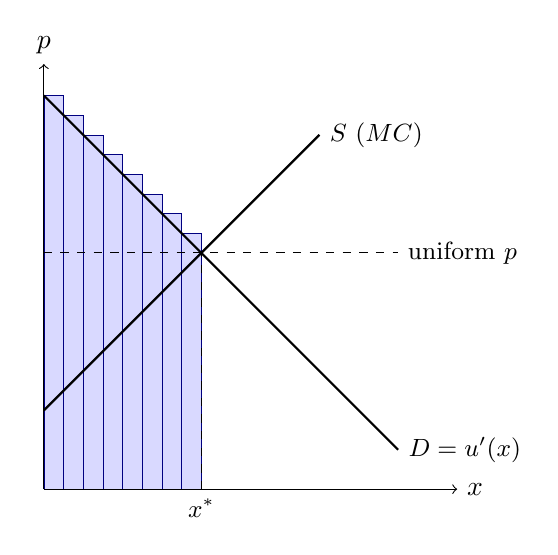
\begin{tikzpicture}[scale=0.5]
\foreach \k in {0,...,7}{
  \pgfmathsetmacro{\xl}{0.5*\k}
  \pgfmathsetmacro{\h}{10-0.5*\k}
  \fill[blue!15] (\xl,0) rectangle ({\xl+0.5},\h);
  \draw[blue!50!black,very thin] (\xl,0) rectangle ({\xl+0.5},\h);
}
\draw[->] (0,0)--(10.5,0) node[right]{$x$};
\draw[->] (0,0)--(0,10.8) node[above]{$p$};
\draw[thick] (0,10)--(9,1) node[right]{\small $D=u'(x)$};
\draw[thick] (0,2)--(7,9) node[right]{\small $S$ ($MC$)};
\draw[dashed] (0,6)--(9,6) node[right]{\small uniform $p$};
\draw[dashed] (4,0) node[below]{\small $x^*$}--(4,6);
\end{tikzpicture}
\end{center}
\textit{How to read the figure.} The shaded strips are the per-unit prices $p_1,p_2,\dots$ under per-unit pricing; each strip's height is the willingness to pay for that piece. Their total area is the area under the demand curve up to $x^*$, $u(x^*)$, which is also the bundle price. Under uniform pricing the consumer pays only the horizontal line $p$ on every unit and keeps the area between demand and that line.

\paragraph{Second-degree price discrimination (nonlinear pricing).} The firm's revenue is a nonlinear function of the amount purchased (e.g.\ quantity discounts). With two consumers, $u_1(x_1)+y_1$ (low demand) and $u_2(x_2)+y_2$ (high demand), the assumption above that the consumer with the larger \emph{total} willingness to pay also has the larger \emph{marginal} willingness to pay ($u_2>u_1$ and $u_2'>u_1'$) is known as the \textbf{single-crossing property}. It is what lets the seller design a menu of (quantity, payment) bundles that the two types choose between voluntarily (self-selection). The full second-degree analysis is not developed in these notes.

%======================================================================
\subsection{Third-degree price discrimination \pg{59--61}}

\paragraph{Setup.}
\begin{itemize}
\item Two identifiable groups (markets) $i=1,2$; the firm can enforce the division (e.g.\ by age for discounts), so there is no resale.
\item $p_i(x_i)$: inverse demand of group $i$; $x_i$ is the quantity sold to group $i$.
\item Constant marginal cost $c$.
\item Elasticity in market $i$: $\epsilon_i=\dfrac{dx_i}{dp_i}\dfrac{p_i}{x_i}<0$, written $|\epsilon_i|$ in absolute value.
\end{itemize}
Within each group every unit sells at one price, but the prices can differ across groups.

\paragraph{Separate markets.} The firm solves
\[
\max_{x_1,x_2}\ p_1(x_1)\,x_1+p_2(x_2)\,x_2-cx_1-cx_2 .
\]
The objective is additively separable, so each market is a separate monopoly problem. FOCs:
\begin{align*}
p_1(x_1)+p_1'(x_1)\,x_1&=c, & p_2(x_2)+p_2'(x_2)\,x_2&=c .
\end{align*}
Rewrite each in elasticity form exactly as in \eqref{eq:micro-markup}:
\begin{equation}\label{eq:micro-3rd}
p_1(x_1)\Big[1-\frac{1}{|\epsilon_1|}\Big]=c,\qquad p_2(x_2)\Big[1-\frac{1}{|\epsilon_2|}\Big]=c .
\end{equation}
Both left-hand sides equal $c$, so $p_1\big[1-1/|\epsilon_1|\big]=p_2\big[1-1/|\epsilon_2|\big]$, i.e.
\[
\frac{p_1}{p_2}=\frac{1-1/|\epsilon_2|}{1-1/|\epsilon_1|}.
\]
The right side exceeds $1$ iff $1-1/|\epsilon_2|>1-1/|\epsilon_1|$ iff $|\epsilon_2|>|\epsilon_1|$.

\begin{keybox}[title=Inverse-elasticity rule]
\[
p_1>p_2\iff|\epsilon_1|<|\epsilon_2| .
\]
The market with the more elastic demand (the more price-sensitive group) is charged the lower price.
\end{keybox}

\paragraph{Linked markets.} Suppose the firm cannot separate the markets cleanly, so the quantity sold in one market affects willingness to pay in the other: $p_i=p_i(x_1,x_2)$. The firm solves
\[
\max_{x_1,x_2}\ p_1(x_1,x_2)\,x_1+p_2(x_1,x_2)\,x_2-cx_1-cx_2 .
\]
Now $x_1$ affects revenue in market 2 as well. FOCs:
\begin{align*}
\frac{\partial}{\partial x_1}:\quad p_1+\frac{\partial p_1}{\partial x_1}\,x_1+\frac{\partial p_2}{\partial x_1}\,x_2&=c,\\
\frac{\partial}{\partial x_2}:\quad p_2+\frac{\partial p_2}{\partial x_2}\,x_2+\frac{\partial p_1}{\partial x_2}\,x_1&=c.
\end{align*}
Defining the own-market elasticity by $\frac{1}{\epsilon_i}=\frac{\partial p_i}{\partial x_i}\frac{x_i}{p_i}$ and factoring $p_i$ out of the first two terms, as before:
\begin{align}
p_1\Big[1-\frac{1}{|\epsilon_1|}\Big]+\frac{\partial p_2}{\partial x_1}\,x_2&=c, \label{eq:micro-link1}\\
p_2\Big[1-\frac{1}{|\epsilon_2|}\Big]+\frac{\partial p_1}{\partial x_2}\,x_1&=c. \label{eq:micro-link2}
\end{align}
\emph{Symmetry of cross effects.} With quasilinear utility $u(x_1,x_2)+y$, the inverse demands are $p_i=\partial u/\partial x_i$, so (Young's theorem: cross-partials are equal)
\[
\frac{\partial p_1}{\partial x_2}=\frac{\partial^2u}{\partial x_2\,\partial x_1}=\frac{\partial^2u}{\partial x_1\,\partial x_2}=\frac{\partial p_2}{\partial x_1}\equiv u_{12}.
\]
Subtract \eqref{eq:micro-link2} from \eqref{eq:micro-link1} and use this symmetry:
\begin{align*}
p_1\Big[1-\tfrac{1}{|\epsilon_1|}\Big]-p_2\Big[1-\tfrac{1}{|\epsilon_2|}\Big]+u_{12}\,x_2-u_{12}\,x_1&=0\\
p_1\Big[1-\tfrac{1}{|\epsilon_1|}\Big]-p_2\Big[1-\tfrac{1}{|\epsilon_2|}\Big]&=(x_1-x_2)\,\frac{\partial p_2}{\partial x_1}.
\end{align*}

\emph{Sign of the cross effect.} The two groups buy the same good, so it is natural to treat the two ``goods'' as \textbf{substitutes}: selling more to group 1 lowers group 2's willingness to pay, $\partial p_2/\partial x_1=u_{12}<0$. (Formally: inverting the inverse demands, $\partial x_1/\partial p_2=-u_{12}/\det H$ where $H$ is the Hessian of $u$, with $\det H>0$ by strict concavity; substitutes, $\partial x_1/\partial p_2>0$, means $u_{12}<0$.)

Now suppose $x_1>x_2$. Then the right-hand side $(x_1-x_2)\,u_{12}<0$, so
\begin{align*}
p_1\Big[1-\tfrac{1}{|\epsilon_1|}\Big]&<p_2\Big[1-\tfrac{1}{|\epsilon_2|}\Big]\\
\frac{p_1}{p_2}&<\frac{1-1/|\epsilon_2|}{1-1/|\epsilon_1|} &&\text{(divide by $p_2[1-1/|\epsilon_1|]>0$).}
\end{align*}
If $|\epsilon_1|>|\epsilon_2|$, then $1-1/|\epsilon_1|>1-1/|\epsilon_2|$, the right side is below $1$, and therefore $p_1<p_2$.

\emph{Interpretation:} as with separate markets, the more elastic market (here market 1, which also buys more) gets the lower price. The cross effect matters for the exact prices, but with substitutes it does not overturn the inverse-elasticity ranking.

\paragraph{Welfare effect: setup.}
\begin{itemize}
\item Two groups summarized by quasilinear utility $u(x_1,x_2)+y$ with $u$ concave, so $p_i(x_1,x_2)=\partial u(x_1,x_2)/\partial x_i$.
\item $c(x_1,x_2)$: cost of providing $x_1$ and $x_2$. Social welfare $W(x_1,x_2)=u(x_1,x_2)-c(x_1,x_2)$.
\item Two situations to compare: an initial one $(x_1^0,x_2^0)$ with prices $(p_1^0,p_2^0)$, and a new one $(x_1',x_2')$ with prices $(p_1',p_2')$. Write $\Delta x_i=x_i'-x_i^0$, $\Delta u=u(x')-u(x^0)$, $\Delta c$, $\Delta W=\Delta u-\Delta c$.
\end{itemize}
\emph{Question:} does moving to third-degree price discrimination raise social welfare?

\paragraph{Bounds on $\Delta u$.} Apply the concavity inequality (a concave function lies below its tangent plane) twice.
\begin{itemize}
\item Tangent plane at $x^0$, evaluated at $x'$:
\begin{align*}
u(x_1',x_2')&\le u(x_1^0,x_2^0)+\frac{\partial u(x^0)}{\partial x_1}(x_1'-x_1^0)+\frac{\partial u(x^0)}{\partial x_2}(x_2'-x_2^0)\\
\Delta u&\le p_1^0\,\Delta x_1+p_2^0\,\Delta x_2 &&\text{(use $p_i^0=\partial u(x^0)/\partial x_i$).}
\end{align*}
\item Tangent plane at $x'$, evaluated at $x^0$:
\begin{align*}
u(x_1^0,x_2^0)&\le u(x_1',x_2')+p_1'\,(x_1^0-x_1')+p_2'\,(x_2^0-x_2')\\
\Delta u&\ge p_1'\,\Delta x_1+p_2'\,\Delta x_2 &&\text{(rearrange; flip signs).}
\end{align*}
\end{itemize}
Subtract $\Delta c$ throughout:
\[
p_1^0\,\Delta x_1+p_2^0\,\Delta x_2-\Delta c\ \ge\ \Delta W\ \ge\ p_1'\,\Delta x_1+p_2'\,\Delta x_2-\Delta c .
\]
With constant marginal cost, $\Delta c=c\,\Delta x_1+c\,\Delta x_2$, so
\begin{equation}\label{eq:micro-wbounds}
(p_1^0-c)\,\Delta x_1+(p_2^0-c)\,\Delta x_2\ \ge\ \Delta W\ \ge\ (p_1'-c)\,\Delta x_1+(p_2'-c)\,\Delta x_2 .
\end{equation}

\paragraph{Applying the bounds to price discrimination.} Let the initial situation be uniform monopoly pricing (no discrimination), $p_1^0=p_2^0=p^0$, and let $(p_1',p_2')$ be the discriminatory prices. Then \eqref{eq:micro-wbounds} becomes
\[
(p^0-c)\,(\Delta x_1+\Delta x_2)\ \ge\ \Delta W\ \ge\ (p_1'-c)\,\Delta x_1+(p_2'-c)\,\Delta x_2 .
\]
\begin{itemize}
\item \textbf{Upper bound.} A monopolist prices above marginal cost, $p^0-c>0$. If total output fell, $\Delta x_1+\Delta x_2<0$, the upper bound would be negative and so $\Delta W<0$. Hence welfare can rise only if total output rises.
\item \textbf{Lower bound.} If the price-cost-weighted sum of output changes is positive, then $\Delta W$ is above a positive number, so welfare rises.
\end{itemize}
\begin{keybox}[title=Welfare effect of third-degree price discrimination]
\begin{itemize}
\item \textbf{Necessary} for $\Delta W>0$: total output increases, $\Delta x_1+\Delta x_2>0$.
\item \textbf{Sufficient} for $\Delta W>0$: $\sum_i(p_i'-c)\,\Delta x_i>0$.
\end{itemize}
\end{keybox}
\emph{Interpretation:} discrimination moves units from one group to the other. At the uniform price every unit has the same marginal value $p^0$, so merely reshuffling a fixed total cannot help; welfare can rise only if discrimination expands total sales (e.g.\ by opening a market that the uniform price left unserved).

\paragraph{Example: linear demands, zero marginal cost.} Let $x_i=a_i-b_ip_i$ ($a_i,b_i>0$), so $p_i(x_i)=(a_i-x_i)/b_i$, and let $c=0$.

\emph{With discrimination,} the firm maximizes revenue in each market separately:
\begin{align*}
&\max_{x_i}\ R_i(x_i)=\frac{a_i-x_i}{b_i}\,x_i=\frac{a_ix_i-x_i^2}{b_i}\\
&\frac{dR_i}{dx_i}=\frac{a_i-2x_i}{b_i}=0 &&\text{(FOC, $MR=MC=0$)}\\
&x_i=\frac{a_i}{2},\qquad x_1+x_2=\frac{a_1+a_2}{2}.
\end{align*}
\emph{Without discrimination,} the firm chooses one price $p$ for both markets:
\begin{align*}
&R(p)=p\,(x_1+x_2)=p\big[(a_1-b_1p)+(a_2-b_2p)\big]=(a_1+a_2)\,p-(b_1+b_2)\,p^2\\
&R'(p)=(a_1+a_2)-2(b_1+b_2)\,p=0 &&\text{(FOC)}\\
&p^*=\frac{a_1+a_2}{2(b_1+b_2)} &&\text{(solve for $p$)}\\
&x_1+x_2=(a_1+a_2)-(b_1+b_2)\,p^*=(a_1+a_2)-\frac{a_1+a_2}{2}=\frac{a_1+a_2}{2}. &&\text{(substitute)}
\end{align*}
Total output is the same under both regimes, $\Delta x_1+\Delta x_2=0$. By the upper bound, $\Delta W\le(p^0-c)\cdot 0=0$.

\begin{keybox}[title=Linear demand result]
With linear demands and both markets served at the uniform price (i.e.\ $a_i-b_ip^*\ge 0$ for $i=1,2$), third-degree price discrimination leaves total output unchanged and therefore cannot raise welfare: $\Delta W\le 0$ (typically $<0$, because output is misallocated across the groups).
\end{keybox}
